% Hoja de trabajo del taller Hands-On AI, FIT 2026.
%
% Las dos figuras (mundo.pdf y bigramas.pdf) las genera
%   slides/figuras/construir_figuras.py
% No se dibujan a mano.
%
% Se compila con:  pdflatex hoja_de_trabajo.tex
% Son dos paginas: se imprime en una hoja, a doble cara.
\documentclass[10pt,a4paper]{article}

\usepackage[utf8]{inputenc}
\usepackage[T1]{fontenc}
\usepackage[spanish,es-noquoting]{babel}
\usepackage[margin=14mm]{geometry}
\usepackage{tgheros}
\renewcommand{\familydefault}{\sfdefault}
\usepackage{amsmath}
\usepackage{array}
\usepackage{graphicx}
\usepackage{xcolor}
\usepackage{titlesec}
\usepackage{enumitem}

% Colores ETH, los mismos del deck y de los notebooks.
\definecolor{ETHBlue}{HTML}{215CAF}
\definecolor{ETHRed}{HTML}{B7352D}
\definecolor{ETHGreen}{HTML}{8E9C1E}
\definecolor{ETHGray}{HTML}{6F6F6F}

\titleformat{\section}{\large\bfseries\color{ETHBlue}}{\thesection.}{0.5em}{}
\titlespacing{\section}{0pt}{6pt}{4pt}
\setlist[itemize]{leftmargin=14pt,itemsep=2pt,topsep=3pt}
\pagestyle{empty}

\newcommand{\celda}{\rule{0pt}{5.2ex}}

\newcommand{\cabecera}{%
  \noindent
  {\Large\bfseries Hands-On AI \;\textcolor{ETHGray}{\textbar}\; hoja de trabajo}
  \hfill
  {\color{ETHGray}\small FIT 2026 \quad Nombre: \rule{45mm}{0.4pt}}
  \vspace{2pt}
  \noindent\textcolor{ETHBlue}{\rule{\textwidth}{1pt}}
}

\newcommand{\piedepagina}{%
  \vfill
  \noindent\textcolor{ETHBlue}{\rule{\textwidth}{0.4pt}}
  \noindent{\color{ETHGray}\scriptsize
  Taller Hands-On AI \textbullet\ Dr.\ Leonel Aguilar, ETH Z\"urich \textbullet\
  Notebooks y soluciones: \texttt{github.com/leaguilar/fit\_2026}}
}

\begin{document}

% ==================================================================
%  PAGINA 1: LA Q-TABLE
% ==================================================================
\cabecera

\section{La Q-table, a mano}

El agente vive en cinco casillas y quiere comer. Nadie le dijo d\'onde est\'a
la comida: lo tiene que descubrir solo.

\begin{center}
  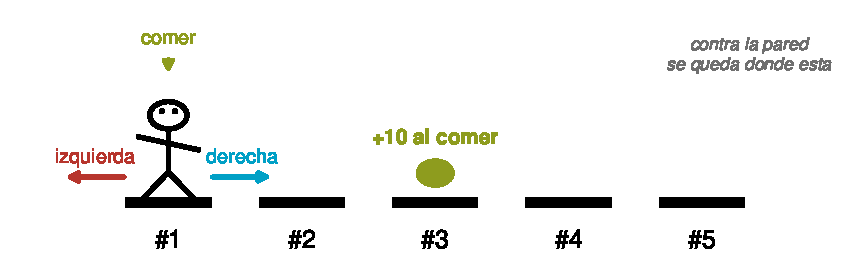
\includegraphics[width=0.80\textwidth]{mundo.pdf}
\end{center}

\vspace{-4pt}
\noindent\textbf{La regla (ecuaci\'on de Bellman), con $\gamma = 0{,}1$:}
\begin{equation*}
Q(s,a) \;=\; \underbrace{r}_{\text{el premio de ahora}}
\;+\; 0{,}1 \cdot \underbrace{\max_{a'} Q(s',a')}_{\text{lo mejor que puedes hacer despu\'es}}
\end{equation*}

\vspace{-4pt}
\noindent\textbf{Empieza por lo m\'as f\'acil.} Despu\'es de comer sigues en la
\#3, y lo mejor que puedes hacer es volver a comer:
\[
Q(\#3,\text{comer}) = 10 + 0{,}1 \cdot Q(\#3,\text{comer})
\quad\Longrightarrow\quad
Q(\#3,\text{comer}) = \underline{\hspace{20mm}}
\]

\vspace{-6pt}
\noindent Y desde ah\'i hacia afuera:\quad
$Q(\#2,\text{derecha}) = 0 + 0{,}1 \cdot \underline{\hspace{16mm}}
= \underline{\hspace{16mm}}$

\vspace{6pt}
\begin{center}
\setlength{\tabcolsep}{12pt}
\begin{tabular}{|l|c|c|c|}
\hline
\rule{0pt}{3.4ex} \textbf{estado} &
\textcolor{ETHRed}{\textbf{izquierda}} &
\textbf{derecha} &
\textcolor{ETHGreen}{\textbf{comer}} \\
\hline
\celda \#1 & & & \\ \hline
\celda \#2 & & & \\ \hline
\celda \#3 \small(comida) & & & \\ \hline
\celda \#4 & & & \\ \hline
\celda \#5 & & & \\ \hline
\end{tabular}
\end{center}

\vspace{2pt}
\noindent\textbf{Cuando termines:} rodea con un c\'irculo el n\'umero m\'as
grande de cada fila. Esa columna es la \textbf{estrategia} del agente.

\vspace{4pt}
\noindent{\color{ETHGray}\small
¿Tiene sentido? ¿Qu\'e hace el agente si empieza en la \#5?}
\rule{75mm}{0.4pt}

\piedepagina
\newpage

% ==================================================================
%  PAGINA 2: LOS BIGRAMAS
% ==================================================================
\cabecera

\section{La tabla de bigramas, a mano}

Un modelo de lenguaje predice la siguiente palabra. La forma m\'as simple de
hacerlo es \textbf{contar}: para cada palabra, apunta qu\'e palabras vinieron
despu\'es y cu\'antas veces.

\begin{center}
  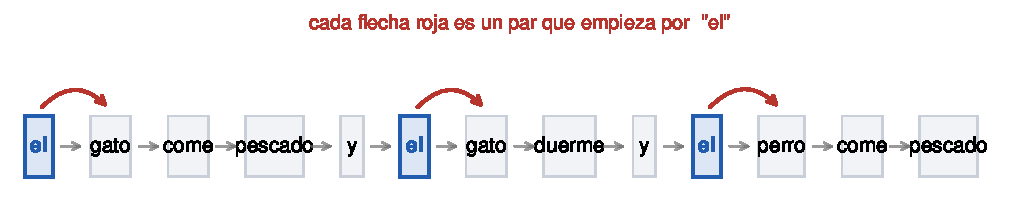
\includegraphics[width=1.0\textwidth]{bigramas.pdf}
\end{center}

\vspace{-6pt}
\noindent Ejemplo: despu\'es de \texttt{el} viene \texttt{gato} dos veces y
\texttt{perro} una. Completa el resto.

\vspace{6pt}
\begin{center}
\setlength{\tabcolsep}{12pt}
\begin{tabular}{|l|p{100mm}|}
\hline
\rule{0pt}{3.4ex} \textbf{despu\'es de\ldots} &
\textbf{\ldots viene (palabra y cu\'antas veces)} \\
\hline
\celda \texttt{el}      & \\ \hline
\celda \texttt{gato}    & \\ \hline
\celda \texttt{come}    & \\ \hline
\celda \texttt{pescado} & \\ \hline
\celda \texttt{y}       & \\ \hline
\celda \texttt{duerme}  & \\ \hline
\celda \texttt{perro}   & \\ \hline
\end{tabular}
\end{center}

\vspace{4pt}
\noindent\textbf{Tres preguntas:}
\begin{itemize}
  \item Si el modelo acaba de escribir \texttt{el}, ¿qu\'e palabra elige?
        ¿Con qu\'e probabilidad? \rule{55mm}{0.4pt}
  \item Fíjate en la \textbf{forma} de esta tabla y en la de la otra cara.
        ¿En qu\'e se parecen? \rule{55mm}{0.4pt}
  \item ¿Cu\'antas filas tendr\'ia esta tabla si en vez de una palabra
        mir\'aramos las \textbf{tres} anteriores? \rule{40mm}{0.4pt}
\end{itemize}

\vspace{4pt}
\noindent{\color{ETHRed}\small\textbf{Esa \'ultima pregunta es la del taller.}
Cuantas m\'as palabras de contexto, m\'as filas, y menos ejemplos por fila.
Ah\'i es donde la tabla se rompe y hace falta una red.}

\piedepagina

\end{document}
